\documentclass[11pt,twoside]{article}

\usepackage[letterpaper,margin=1in]{geometry}
\usepackage{microtype}
\usepackage{amsmath,amssymb}
\usepackage{newtxtext}
\usepackage[amsthm]{newtxmath}
\usepackage{booktabs}
\usepackage{enumitem}
\usepackage{fancyhdr}
\usepackage{xcolor}
\usepackage{tcolorbox}
\usepackage{tikz}
\usetikzlibrary{arrows.meta,positioning}
\usepackage[colorlinks=true,linkcolor=InkNavy,citecolor=MutedTeal,urlcolor=MutedTeal]{hyperref}
\usepackage[nameinlink,capitalise]{cleveref}

\definecolor{InkNavy}{HTML}{18324A}
\definecolor{MutedTeal}{HTML}{2F6F73}
\definecolor{WarmPaper}{HTML}{FBFAF6}
\definecolor{BoxTint}{HTML}{EDF4F2}
\pagecolor{WarmPaper}
\color{InkNavy!92!black}

\newtcolorbox{keyidea}{colback=BoxTint,colframe=MutedTeal,title=Key idea}
\newtcolorbox{trustboundary}{colback=InkNavy!4,colframe=InkNavy,title=Trust boundary}
\newtcolorbox{nonclaim}{colback=black!3,colframe=black!55,title=What this does not prove}

\newtheorem{definition}{Definition}[section]
\newtheorem{theorem}[definition]{Theorem}
\newtheorem{lemma}[definition]{Lemma}
\newtheorem{proposition}[definition]{Proposition}
\newtheorem{example}[definition]{Example}
\theoremstyle{remark}
\newtheorem{remark}[definition]{Remark}

\pagestyle{fancy}
\fancyhf{}
\fancyhead[LE]{\small\textsc{Proof-Producing Base-19 Obstruction}}
\fancyhead[RO]{\small\textsc{8128}}
\fancyfoot[C]{\thepage}
\setlength{\headheight}{14pt}

\hypersetup{
  pdftitle={A Proof-Producing Base-19 Obstruction in a Reverse-and-Add Constraint System},
  pdfauthor={8128},
  pdfsubject={Preprint candidate}
}

% Generated; do not edit.
\newcommand{\BaseValue}{19}
\newcommand{\CandidateEquationCount}{409}
\newcommand{\CoreEquationCount}{408}
\newcommand{\RadialLayerCount}{35}
\newcommand{\TerminalLayer}{33}
\newcommand{\PeakReachableStates}{314}
\newcommand{\MaximumFrontierDigits}{2}
\newcommand{\MaximumFrontierCarries}{12}
\newcommand{\ActiveDigitCount}{409}
\newcommand{\ActiveCarryCount}{410}
\newcommand{\DeletionAuditCount}{409}
\newcommand{\SatDeletionCount}{408}
\newcommand{\UnsatDeletionCount}{1}
\newcommand{\RemovedCoreEquation}{\texttt{phase=0,n=0,column=82}}
\newcommand{\KnownSatRemovedEquation}{\texttt{phase=0,n=0,column=0}}
\newcommand{\CoreReplaySeconds}{34.53}
\newcommand{\CertificateGenerationSeconds}{172.90}
\newcommand{\DeletionAuditSeconds}{32677.27}
\newcommand{\CleanCloneSeconds}{245.46}
\newcommand{\LeanWitnessSeconds}{37.60}
\newcommand{\CandidateCertificateSha}{\texttt{1ce1b3c59bd95264e5338f7fba5bdffa15fb7635917964980057615395cf138c}}
\newcommand{\CoreCertificateSha}{\texttt{7635e7188197021cfc15cbad6d087f6fdbfa7a8bbfe4e4ed9b91a15a89498c67}}
\newcommand{\DeletionAuditSha}{\texttt{0566f6e2025aec28fe0d2f824f1f6b343cf912e9191a9036629a2a1d4ef03325}}
\newcommand{\GenericSoundnessTheorem}{\texttt{Base19Radial.unsat\_of\_closed\_empty\_frontier}}
\newcommand{\ConcreteSatTheorem}{\texttt{Base19Radial.deleteP0C0Sat}}
\newcommand{\PackedWidth}{4914}
\newcommand{\PackedSlotWidth}{6}
\newcommand{\PackedConstraintCount}{1233}
\newcommand{\PackedLeanSeconds}{51.01}
\newcommand{\PackedLeanMaxRSS}{1.28\,GB}
\newcommand{\PackedTheorem}{\texttt{Base19Radial.packedMinimalCoreUnsat}}
\newcommand{\PackedManifestSha}{\texttt{18ca75da64c84859d2373ae3e61da81e3ac75a68a33af448b57220e23dfbfa9e}}


\newcommand{\Candidate}{\ensuremath{\mathcal{C}}}
\newcommand{\Core}{\ensuremath{\mathcal{C}^{\circ}}}

\title{A Proof-Producing Base-19 Obstruction in a Reverse-and-Add Constraint System}
\author{8128}
\date{August 2026}

\begin{document}
\maketitle

\begin{abstract}
We study one frozen, finite constraint system extracted from a six-phase
reverse-and-add topology in base~\BaseValue.  Exact radial-frontier replay
ends in the empty set for a \CandidateEquationCount-equation candidate and
for a \CoreEquationCount-equation subset.  A complete one-equation-deletion
audit makes the latter computationally deletion-minimal.  Lean separately
proves the generic implication from a closed empty frontier to
unsatisfiability; the concrete frontier replays remain computational claims.
This bounded obstruction is not a theorem about the unbounded reverse-and-add
process and does not establish a base-19 Lychrel number.
\end{abstract}

\tableofcontents
\clearpage

\section{Orientation}
\label{sec:orientation}

For a base-$b$ numeral, a \emph{reverse-and-add step} adds the represented
integer to the integer represented by the reversed digit word.  Reversal
couples digits at opposite ends, whereas carrying couples adjacent columns.
The elementary operation therefore becomes a globally coupled system when
several steps are required to have a prescribed repeating shape.

\begin{example}[A decimal step]
Take the two-digit decimal word $47$.  Reversing and adding gives
\[
  \begin{array}{r}
      47\\[-2pt]
    + 74\\ \hline
     121
  \end{array}
  \qquad\text{since}\qquad
  \begin{aligned}
    7+4+0 &= 1+10\cdot 1,\\
    4+7+1 &= 2+10\cdot 1,\\
    0+0+1 &= 1+10\cdot 0.
  \end{aligned}
\]
The three equalities are the units, tens, and new leading column.  They also
show why zero boundary atoms and explicit carry variables are convenient:
the same equation describes every column.
\end{example}

The topology studied here was prompted by David Seal's reported period-six,
self-similar base-17 construction, preserved in Brown's account
\cite{brownSeal}.  OEIS A060382 records conjectural least starts of
palindrome-free reverse-and-add sequences by base and cautions that only its
base-two entry is proved \cite{oeisA060382}.  These sources provide motivation
and provenance only.  Neither supplies a premise for the finite base-19
calculation below, and no claim of novelty or resolution of the OEIS entry is
made.

\begin{keyidea}
The question answered here is deliberately finite: does one explicitly
listed family of bounded digit-and-carry equations have a solution?  Opposite
columns are processed together, leaving only a small radial frontier between
the processed exterior and the unprocessed center.
\end{keyidea}

\section{The frozen base-19 system}
\label{sec:frozen-system}

Set $b=\BaseValue$.  Every digit variable has domain
$D=\{0,1,\ldots,18\}$, every carry variable has domain $K=\{0,1\}$, and
the leading digit of each phase is restricted to $D\setminus\{0\}$.  Literal
atoms are fixed integers, not variables.  At phase $p$ and column $k$, write
$\ell_{p,k}$ and $r_{p,k}$ for the source atoms met from the two ends,
$t_{p,k}$ for the target atom, and $c_{p,k-1},c_{p,k}$ for the incoming and
outgoing carries.  A missing end atom or boundary carry is the literal zero.
The exact column constraint is
\begin{equation}
  \ell_{p,k}+r_{p,k}+c_{p,k-1}
  =t_{p,k}+19c_{p,k}.
  \label{eq:base19-column}
\end{equation}
Thus every symbol and every domain in \cref{eq:base19-column} is an ordinary
bounded integer; modular arithmetic enters only in the later packed encoding.

There are six phases $p\in\{0,1,\ldots,5\}$.  Each phase word has three
variable blocks.  Their lengths are
\[
  (26,25,31) \quad\text{for }p=0,
  \qquad
  (29,23,31) \quad\text{for }p=1,\ldots,5.
\]
For $n\geq 0$, insert a constant run of length $n$ between consecutive
blocks.  The two inserted digits are $(0,18)$ for phases $0,2,3,4,5$ and
$(18,0)$ for phase $1$.  Denote the resulting word by $W_p(n)$.

Words are written most-significant digit first.  More formally, let
$s_p=|W_p(0)|$, set $V_p=W_{p+1}(0)$ when $0\leq p<5$ and
$V_5=W_0(1)$, and let $m_p=|V_p|$.  Write these source and target words as
\[
  W_p(0)=x_{p,0}x_{p,1}\cdots x_{p,s_p-1},
  \qquad
  V_p=y_{p,0}y_{p,1}\cdots y_{p,m_p-1}.
\]
The source and target lengths are $s_0=82$, $s_p=83$ for
$1\leq p\leq5$, $m_p=83$ for
$0\leq p<5$, and $m_5=84$.  Arithmetic column $k=0$ is the
least-significant target column.  For $0\leq k<m_p$, the written-index map is
\begin{align}
  \ell_{p,k}
    &=\begin{cases}
        x_{p,k}, & k<s_p,\\
        0, & k\geq s_p,
      \end{cases}
  &
  r_{p,k}
    &=\begin{cases}
        x_{p,s_p-1-k}, & k<s_p,\\
        0, & k\geq s_p,
      \end{cases}
  \label{eq:source-index-map}\\
  t_{p,k}&=y_{p,m_p-1-k}.&&
  \label{eq:target-index-map}
\end{align}
In particular, $\ell_{p,k}$ advances from the written left (most-significant)
end, while $r_{p,k}$ advances from the written right (least-significant) end;
missing source positions are literal zero.  The initial and final boundary
carries are zero:
\begin{equation}
  c_{p,-1}=0,
  \qquad
  c_{p,m_p-1}=0.
  \label{eq:carry-boundaries}
\end{equation}

For $p<5$, phase $p$ therefore imposes the column equations taking $W_p(0)$
to $W_{p+1}(0)$.  Phase $5$ takes $W_5(0)$ to $W_0(1)$; this is the single
growth step that closes the six-phase cycle.  In particular, phase-5 column
83 has target index $m_5-1-83=0$.  Since $83=s_5$, both source atoms are
literal zero, the target is the leading atom \texttt{p0:f0:d0}, and the final
outgoing carry is $c_{5,83}=0$.  Its retained equation is therefore
\begin{equation}
  0+0+c_{5,82}=\texttt{p0:f0:d0}+19\cdot0.
  \label{eq:phase5-growth-column}
\end{equation}
The omitted phase-5 column 82 removes that column equation, but its named
outgoing carry $c_{5,82}$ remains the incoming carry in
\cref{eq:phase5-growth-column}.

Only two exterior coordinate bands from each full addition are retained.
They are
\begin{align*}
  p=0 &: \quad 0\text{--}33 \ \text{and}\ 48\text{--}82,\\
  p=1,2,3,4 &: \quad 0\text{--}33 \ \text{and}\ 49\text{--}82,\\
  p=5 &: \quad 0\text{--}33 \ \text{and}\ 49\text{--}83.
\end{align*}
The builder then omits \texttt{phase=5,n=0,column=82}.  The remaining
equations, in their canonical manifest order, form the frozen candidate
$\Candidate$.  It has exactly \CandidateEquationCount{} equations over
\ActiveDigitCount{} active digit variables and \ActiveCarryCount{} active
carry variables.  Each equation carries a provenance label of the form
\texttt{phase=p,n=0,column=k}; the manifest also fixes every literal,
variable name, and carry endpoint.

Finally let
\[
  e_\star=\text{\RemovedCoreEquation},
  \qquad
  \Core=\Candidate\setminus\{e_\star\}.
\]
Consequently $\Core$ contains \CoreEquationCount{} equations.  This removal
must not be confused with the earlier phase-5 omission used to define the
candidate itself.  The three objects used below are therefore: the
\CandidateEquationCount-equation candidate $\Candidate$, its
\CoreEquationCount-equation subset $\Core$, and the complete audit of every
single-equation deletion of $\Candidate$.

\section{Radial decomposition}
\label{sec:radial-decomposition}

The retained columns are paired from the outside toward the center across all
six phases.  The promoted certificate stores \RadialLayerCount{} atomic
layers, labeled $-1,0,\ldots,\TerminalLayer$.  The label $-1$ is a
one-equation bootstrap layer.  For cleaner notation here, merge that
bootstrap with stored layer $0$ and call the result $L_0$; for
$1\leq i\leq 33$, let $L_i$ be stored layer $i$.  This harmless coarsening
gives the 34 transfers shown in \cref{fig:radial-frontier}.

For a set of equations $E$, let $\operatorname{Var}(E)$ be its variables.
After processing through $L_i$, the live interface is the canonically sorted
list
\begin{equation}
  I_i = \operatorname{Var}(L_0\cup\cdots\cup L_i)
  \cap \operatorname{Var}(L_{i+1}\cup\cdots\cup L_{33}),
  \qquad I_{-1}=().
  \label{eq:live-interface}
\end{equation}
A state on $I_i$ is a domain-respecting tuple in that fixed order.  Put
$H_i=\operatorname{Var}(L_i)\setminus(I_{i-1}\cup I_i)$.  For a state $s$
on $I_{i-1}$, the exact local transfer is
\begin{equation}
  T_i(s)=\left\{u\text{ on }I_i:\
    \begin{array}{l}
      \text{there is a domain-respecting assignment }h\text{ on }H_i,\\[-2pt]
      s,u,h\text{ agree on overlaps and together satisfy every equation in }L_i
    \end{array}
  \right\}.
  \label{eq:local-transfer}
\end{equation}
Starting from the one empty tuple, define the reachable frontiers by
\begin{equation}
  F_{-1}=\{()\},
  \qquad
  F_i=\bigcup_{s\in F_{i-1}}T_i(s)
  \quad(0\leq i\leq 33).
  \label{eq:frontier-recurrence}
\end{equation}
This is exact variable elimination: variables that do not cross the cut are
composed locally and then forgotten.  Its usefulness comes from the bounded
live interface, the same general phenomenon behind path-structured and
bounded-width constraint algorithms \cite{Freuder1990,DechterPearl1989}.
Those references provide methodological context only; they do not verify a
transition or a numerical claim in this artifact.

\begin{figure}[t]
  \centering
  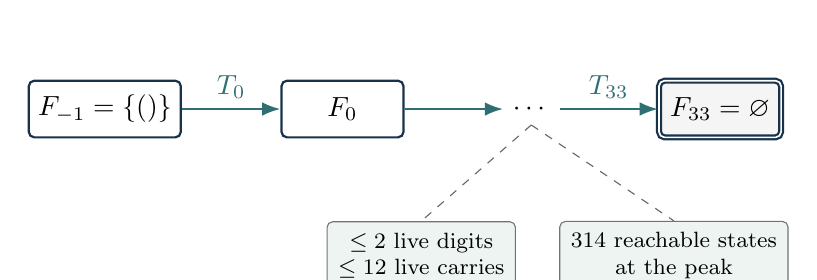
\begin{tikzpicture}[
      >=Latex,
      frontier/.style={draw=InkNavy,rounded corners=2pt,minimum width=1.55cm,
        minimum height=0.72cm,fill=white,thick},
      emptyfrontier/.style={frontier,double,fill=black!4},
      note/.style={draw=black!55,rounded corners=2pt,fill=BoxTint,
        font=\footnotesize,align=center,inner sep=4pt},
      node distance=1.25cm
    ]
    \node[frontier] (start) {$F_{-1}=\{()\}$};
    \node[frontier,right=of start] (l0) {$F_0$};
    \node[right=of l0] (mid) {$\cdots$};
    \node[emptyfrontier,right=of mid] (l33) {$F_{33}=\varnothing$};

    \draw[->,thick,MutedTeal] (start) -- node[above] {$T_0$} (l0);
    \draw[->,thick,MutedTeal] (l0) -- (mid);
    \draw[->,thick,MutedTeal] (mid) -- node[above] {$T_{33}$} (l33);

    \node[note,below=1.05cm of l0,xshift=1.0cm] (interface)
      {$\leq\MaximumFrontierDigits$ live digits\\
       $\leq\MaximumFrontierCarries$ live carries};
    \node[note,right=0.55cm of interface] (states)
      {$\PeakReachableStates$ reachable states\\at the peak};
    \draw[dashed,black!60] (mid.south) -- (interface.north);
    \draw[dashed,black!60] (mid.south) -- (states.north);
  \end{tikzpicture}
  \caption{The radial frontier computation for $\Core$.  The double outline,
  not color alone, marks the empty terminal frontier.  The callouts are
  generated from the frozen core certificate; the drawing is schematic and
  is not itself proof evidence.}
  \label{fig:radial-frontier}
\end{figure}

For $\Core$, the independently replayed transfers satisfy
$F_{33}=\varnothing$.  At every stored cut there are at most
\MaximumFrontierDigits{} live digit variables and
\MaximumFrontierCarries{} live carry variables, and the largest serialized
reachable frontier contains \PeakReachableStates{} states.  These values are
loaded from \texttt{generated-results.tex}, whose renderer checks the frozen
certificate rather than duplicating them as manuscript literals.

Exact equality in \cref{eq:frontier-recurrence} is more than soundness needs.
Call a sequence $G_{-1},G_0,\ldots,G_{33}$ \emph{closed} when
$()\in G_{-1}$ and
\[
  s\in G_{i-1}\ \text{and}\ u\in T_i(s)
  \quad\Longrightarrow\quad u\in G_i
  \qquad(0\leq i\leq 33).
\]

\begin{theorem}[Closed empty frontier]
\label{thm:closed-empty-frontier}
Suppose the layers cover every equation of a bounded constraint problem and
their adjacent interfaces agree.  If $G_{-1},\ldots,G_{33}$ is closed and
$G_{33}=\varnothing$, then the problem has no satisfying assignment.
\end{theorem}

\begin{proof}
If $a$ were a global satisfying assignment, its restriction to the empty
initial interface would lie in $G_{-1}$.  Assume inductively that
$a|_{I_{i-1}}\in G_{i-1}$.  The restriction of $a$ to the variables of
$L_i$ witnesses
$a|_{I_i}\in T_i(a|_{I_{i-1}})$; closure therefore gives
$a|_{I_i}\in G_i$.  At $i=33$ this puts a state in the empty set, a
contradiction.
\end{proof}

Lean proves precisely this generic implication as
\GenericSoundnessTheorem: from layer coverage, an aligned closed chain, an
initial state, and an empty final frontier, it concludes
$\neg\exists a,\,\texttt{Problem.Satisfies}\ a$.  This theorem does not by
itself check the concrete serialized transitions for either $\Candidate$ or
$\Core$.  Nor is there presently a Lean theorem bridging
\texttt{Problem.Satisfies} to the separate packed proposition discussed
later; that integer-to-packed correspondence remains a paper-level boundary.

\section{Deletion-minimal obstruction}
\label{sec:deletion-minimality}

Three computations must be kept distinct.
\begin{enumerate}[leftmargin=*,itemsep=3pt]
  \item The promoted frontier for the full candidate $\Candidate$ covers all
        \CandidateEquationCount{} equations and ends empty.
  \item Removing $e_\star=\RemovedCoreEquation$ gives $\Core$.  Its separate
        promoted frontier covers \CoreEquationCount{} equations and also ends
        empty after exact replay.
  \item The deletion audit has \DeletionAuditCount{} records, one for each
        equation $e\in\Candidate$.  It records \SatDeletionCount{} complete
        satisfying assignments for $\Candidate\setminus\{e\}$ and
        \UnsatDeletionCount{} UNSAT outcome, occurring exactly when
        $e=e_\star$.
\end{enumerate}

For every $e\in\Core$, the audit's assignment for
$\Candidate\setminus\{e\}$ also satisfies the smaller system
$\Core\setminus\{e\}$.  The audit replays each stored digit and carry bound,
leading-digit condition, and retained integer equality.  Combined with the
separate empty-frontier replay for $\Core$, this establishes the following
carefully qualified result.

\begin{proposition}[Computational deletion minimality]
\label{prop:deletion-minimality}
Under the correctness of the frozen manifest parser, the bounded-integer
encoding, and the exact solver answers replayed by the independent checker,
$\Core$ is unsatisfiable and $\Core\setminus\{e\}$ is satisfiable for every
$e\in\Core$.  Thus $\Core$ is deletion-minimal within the frozen candidate.
\end{proposition}

The qualifier ``computational'' is essential here.  The
\CandidateEquationCount-equation empty frontier, the
\CoreEquationCount-equation core replay, and the
\DeletionAuditCount-way deletion audit are frozen and independently rechecked
computational artifacts.  The generic Lean theorem in
Theorem~\ref{thm:closed-empty-frontier} validates the implication from
suitable closure hypotheses, but this section does not claim that Lean
discharges every concrete frontier transition or all deletion witnesses.

\begin{nonclaim}
Deletion-minimal means that no single remaining equation can be removed from
this core while preserving unsatisfiability.  It is \emph{not
minimum-cardinality}: a different, smaller unsatisfiable subset has not been
excluded.  The result gives no uniqueness or all-base theorem, says nothing
about the unbounded reverse-and-add process, and does not establish a base-19
Lychrel number.
\end{nonclaim}

\section{Packed finite encoding}
\label{sec:packed-encoding}

The generated check replaces a tuple of small integers by one bit-vector.
The active variables of $\Core$ occur in the generator's fixed manifest order:
first the \ActiveDigitCount{} digit variables, then the \ActiveCarryCount{}
carry variables.  Thus there are
\[
  \ActiveDigitCount+\ActiveCarryCount=819
\]
slots.  Each slot has width \PackedSlotWidth{}, so the complete assignment is
a word
\[
  A\in\operatorname{BitVec}(819\cdot\PackedSlotWidth)
    =\operatorname{BitVec}(\PackedWidth).
\]
For $0\leq j<819$, slot $j$ is the unsigned six-bit value extracted from
the bit interval beginning at least-significant-bit offset $6j$.  In the
generated Lean source this operation is
\texttt{assignment.extractLsb' (index * 6) 6}.  The 819 intervals are
disjoint and exhaust all \PackedWidth{} bits; there are no padding bits.

Write $s_j(A)\in\{0,\ldots,63\}$ for the ordinary representative of the
$j$th slot.  Let $\mathsf{PackedCore}_{408}(A)$ be the conjunction emitted by
the deterministic renderer.  Its \PackedConstraintCount{} conjuncts divide
into four audited categories:
\begin{center}
  \begin{tabular}{@{}lr@{}}
    \toprule
    Constraint category & Count \\
    \midrule
    Unsigned digit bounds $s_j(A)<19$ & 409 \\
    Unsigned carry bounds $s_j(A)<2$ & 410 \\
    Nonzero leading digits $s_j(A)\neq0$ & 6 \\
    Retained column equations & 408 \\
    \midrule
    Total & $409+410+6+408=\PackedConstraintCount$ \\
    \bottomrule
  \end{tabular}
\end{center}
The six extra inequalities select the variables
\texttt{p0:f0:d0},\ldots,\texttt{p5:f0:d0}; each already has a digit-bound
conjunct.  Literal atoms and boundary carries remain six-bit constants rather
than occupying slots.  Every retained instance of
\cref{eq:base19-column} is translated literally, with six-bit addition and
multiplication, and hence is initially an equality modulo $64$.

\begin{proposition}[Paper equivalence; unformalized bridge]
\label{prop:packed-equivalence}
The bounded integer assignments satisfying $\Core$ are in bijection with the
words $A:\operatorname{BitVec}(\PackedWidth)$ satisfying
$\mathsf{PackedCore}_{408}(A)$.
\end{proposition}

\begin{proof}
This is a paper proof, not a theorem currently present in Lean.  Consider one
column and take the ordinary representatives of its five atoms.  The bounds
give
\[
  0\leq \ell,r,t\leq18,
  \qquad c_{\rm in},c_{\rm out}\in\{0,1\}.
\]
Consequently
\[
  0\leq\ell+r+c_{\rm in}\leq18+18+1=37,
  \qquad
  0\leq t+19c_{\rm out}\leq18+19=37.
\]
Both sides therefore lie in $[0,37]$.  Since \texttt{37<64}, two such
representatives are equal in $\mathbb Z/64\mathbb Z$ exactly when they are
equal as ordinary integers: their difference is a multiple of $64$ with
absolute value strictly below $64$, and hence is zero.  This proves the
slotwise equivalence of each bit-vector column equation and
\cref{eq:base19-column}; it also shows explicitly that no six-bit operation
in a satisfied column can wrap.

For completeness, let $(v_0,\ldots,v_{818})$ be a tuple of slot values in
$\{0,\ldots,63\}$ and pack it as the \PackedWidth-bit word represented by
\[
  \operatorname{pack}(v)=\sum_{j=0}^{818}v_j2^{6j}.
\]
Six-bit extraction gives
$s_j(\operatorname{pack}(v))=v_j$.  Conversely, because the extracted blocks
partition the entire word,
$\operatorname{pack}(s_0(A),\ldots,s_{818}(A))=A$ for every $A$.  Thus
packing and unpacking are inverse operations.  An integer model supplies
slot values in the required ranges, its six leading digits remain nonzero,
and its integer equations imply the modular ones.  In the other direction,
the unsigned slot bounds recover digits in $\{0,\ldots,18\}$ and carries in
$\{0,1\}$; the nonzero clauses recover the six leading conditions; and the
no-wrap argument recovers every integer equation.  The two constructions
therefore restrict to the claimed bijection of satisfying assignments.
\end{proof}

The renderer constructs and audits this correspondence against the frozen
manifest and records its digest as \PackedManifestSha.  The proposition above
is nevertheless an \emph{unformalized bridge}: no existing Lean declaration
maps the earlier \texttt{Problem.Satisfies} predicate to
$\mathsf{PackedCore}_{408}$.  The generic frontier theorem, this generated
and audited bridge, and the packed theorem below are separate statements.

\section{Proof-producing Lean/LRAT check}
\label{sec:lean-lrat}
Abbreviating the generated conjunction just defined, the exact conclusion of
the generated Lean declaration is as follows.

\begin{tcolorbox}[colback=BoxTint,colframe=MutedTeal,title={Lean theorem:
packed core UNSAT}]
\PackedTheorem{} has type
\[
  \forall A:\operatorname{BitVec}(\PackedWidth),
  \qquad \neg\mathsf{PackedCore}_{408}(A).
\]
Equivalently, no \PackedWidth-bit word satisfies the exact inline conjunction
of \PackedConstraintCount{} generated constraints.
\end{tcolorbox}

At the frozen Lean 4.32.2 source commit, \texttt{bv\_decide} reflects and
bit-blasts the proposition, CaDiCaL performs certificate search, and Lean
passes the resulting LRAT certificate to its proved-sound LRAT checker.  The
Lean implementation, the primary LRAT account, and official CaDiCaL
source/release are cited here at the point of use
\cite{leanBVDecide432,CruzFilipeEtAl2017,cadical301}.  In particular, it is
CaDiCaL in this route---not Z3---that searches for the certificate.

There is a second, essential layer to the checking story.  Lean's checker has
a proved soundness theorem, but the frozen implementation's
\texttt{LratCert.toReflectionProof} uses \texttt{nativeEqTrue} to evaluate the
checker result.  That evaluation contributes an additional dependency to the
accepted theorem term.  The artifact's \texttt{\#print axioms} output reports
the ordinary axiom dependencies
\[
  \texttt{propext},\qquad
  \texttt{Classical.choice},\qquad
  \texttt{Quot.sound},
\]
and the artifact-specific native certificate-evaluation axiom
\begin{center}
  \small\nolinkurl{packedMinimalCoreUnsat._native.bv_decide.ax_1_5}.
\end{center}
Accordingly, the concrete certificate evaluation trusts Lean's native
compiler, code generator, and runtime in addition to the proved checker and
kernel.  The result is proof-producing and substantially narrows the trusted
solver boundary, but it is \emph{not kernel-reduction-only}, not fully
axiom-free, and not an end-to-end formalization of the bounded integer model.

One recorded development-machine run of the generated module took
\PackedLeanSeconds{} seconds and reached \PackedLeanMaxRSS{} maximum resident
set size.  These are measurements of that one run, not a performance
guarantee.  Regeneration compares the source byte-for-byte, checks the
digest binding against the frozen equation manifest, and reruns the
declaration under Lean 4.32.2.  The exact digest is supplied by the generated
results file rather than manually transcribed.

\begin{trustboundary}
Four boundaries must not be collapsed.  Lean proves the generic theorem that
a suitably closed empty frontier implies \texttt{Problem.Satisfies} is
impossible.  The concrete frontier files are instead replayed by exact
computation.  The frozen integer-to-packed translation is generated and
audited but remains the unformalized bridge proved only on paper in
Proposition~\ref{prop:packed-equivalence}.  Finally, \PackedTheorem{} proves
UNSAT for the exact packed proposition, with the native evaluation dependency
listed above.  Therefore the paper does not claim a single end-to-end Lean
theorem from the frozen integer problem to the packed conclusion.
\end{trustboundary}

\section{Assurance ladder}
\label{sec:assurance-ladder}

The preceding distinctions can be arranged by the scope of their trusted
base.  The bottom level re-executes the concrete frontier computation using
Z3's mathematical integers and exact finite comparisons
\cite{z3Arithmetic}; it does not attribute a proof object to Z3.  The middle
level is the achieved packed theorem whose CaDiCaL LRAT certificate is checked
in Lean with native evaluation.  A strict concrete proof checked only by
kernel reduction would be a further endpoint, not a property of the present
artifact.

\begin{figure}[t]
  \centering
  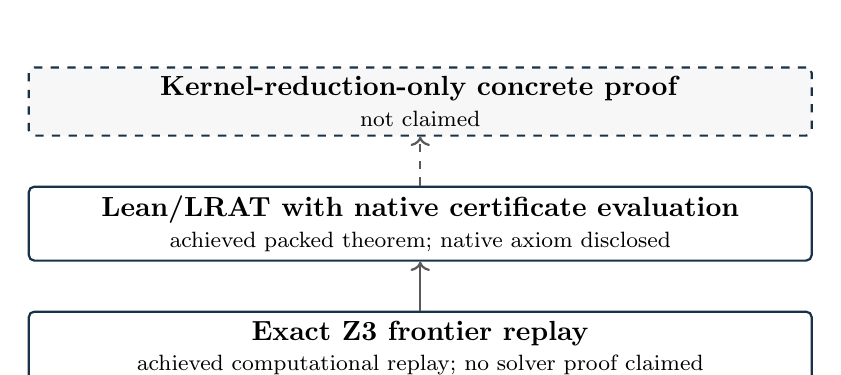
\begin{tikzpicture}[
      level/.style={draw=InkNavy,thick,rounded corners=2pt,
        minimum width=0.82\textwidth,minimum height=0.8cm,
        align=center,fill=white},
      unclaimed/.style={level,dashed,fill=black!3},
      node distance=0.62cm
    ]
    \node[level] (replay)
      {\textbf{Exact Z3 frontier replay}\\[-1pt]
       \footnotesize achieved computational replay; no solver proof claimed};
    \node[level,above=of replay] (native)
      {\textbf{Lean/LRAT with native certificate evaluation}\\[-1pt]
       \footnotesize achieved packed theorem; native axiom disclosed};
    \node[unclaimed,above=of native] (kernel)
      {\textbf{Kernel-reduction-only concrete proof}\\[-1pt]
       \footnotesize not claimed};

    \draw[->,thick,black!65] (replay.north) -- (native.south);
    \draw[->,thick,dashed,black!65] (native.north) -- (kernel.south);
  \end{tikzpicture}
  \caption{Assurance ladder for the concrete checks.  Solid outlines mark
  achieved levels; the dashed outline marks the unclaimed endpoint.  Height
  indicates assurance scope, not mathematical generality.  The diagram is
  explanatory and is not itself proof evidence.}
  \label{fig:assurance-ladder}
\end{figure}

In particular, moving upward in \cref{fig:assurance-ladder} must not be read
as enlarging the theorem's domain.  The frontier replay concerns the frozen
bounded integer instance, while the Lean result concerns its separately
generated packed proposition.  Their correspondence is supplied by the paper
proof and audited renderer, not by a hidden claim that the packed theorem also
formalizes the frontier certificates.

\section{Reproducibility and limitations}
\label{sec:reproducibility}
The generated evidence macros are loaded from \texttt{generated-results.tex}.

\section{Related work and conclusion}
\label{sec:conclusion}
Related-work discussion and the conservative conclusion are deferred.

\appendix
\section{Reproducibility record}
\label{app:reproducibility}
This compact appendix will record theorem names, hashes, and commands.

\bibliographystyle{alpha}
\bibliography{references}

\end{document}
